%% Template article for Elsevier's document class `elsarticle'
%% with numbered style bibliographic references
\documentclass[preprint,12pt]{elsarticle}

% remove preprint footnote
\makeatletter
\def\ps@pprintTitle{%
 \let\@oddhead\@empty
 \let\@evenhead\@empty
 \def\@oddfoot{\centerline{\thepage}}%
 \let\@evenfoot\@oddfoot}
\makeatother


\usepackage{setspace}
\doublespacing

\usepackage[hidelinks]{hyperref} % auto detect ref type
\usepackage{natbib}
\setcitestyle{authoryear}

%% Use the option review to obtain double line spacing
%% \documentclass[preprint,review,12pt]{elsarticle}

%% Use the options 1p,twocolumn; 3p; 3p,twocolumn; 5p; or 5p,twocolumn
%% for a journal layout:
%% \documentclass[final,1p,times]{elsarticle}
%% \documentclass[final,1p,times,twocolumn]{elsarticle}
%% \documentclass[final,3p,times]{elsarticle}
%% \documentclass[final,3p,times,twocolumn]{elsarticle}
%% \documentclass[final,5p,times]{elsarticle}
%% \documentclass[final,5p,times,twocolumn]{elsarticle}

\usepackage{graphicx}
\usepackage{amssymb}
\usepackage{amsmath}
\usepackage{enumerate}
\usepackage{caption}
\usepackage{textcomp}    % for Hawaii characters
%\usepackage{listings}
%\lstset{language=R}
\usepackage[T1]{fontenc}  % tilde in middle in lstlisting
\usepackage[formats]{listings}
\lstset{language=R,
		basicstyle=\ttfamily,
		columns=fixed,
		basewidth=0.5em,
		literate={~}{{$\sim$}}1
		}

\biboptions{comma,round}

% shortcuts
\newcommand{\bbeta}{\boldsymbol{\beta}}
\newcommand{\blambda}{\boldsymbol{\lambda}}
\newcommand{\T}{\intercal}
\newcommand{\bS}{\mathbf{S}}
\newcommand{\bQ}{\mathbf{Q}}
\newcommand{\bSigma}{\boldsymbol{\Sigma}}
\newcommand{\bm}{\boldsymbol}  % bold maths symbols
\newcommand{\tl}{\tilde{\lambda}}   % thinned little lambda
\newcommand{\tL}{\tilde{\Lambda}}  % thinned big lambda

% RJC 09/08/2019 Added shortcuts for Hawaiian words
\newcommand{\akepa}{\textquotesingle\={a}kepa}  % adds Hawaiian diacritical marks
\newcommand{\Akepa}{\textquotesingle\={A}kepa}  % adds Hawaiian diacritical marks
\newcommand{\hawaii}{Hawai\textquotesingle i}   % adds Hawaiian diacritical marks
\DeclareMathOperator*{\argmax}{arg\,max}  % * means _ puts thing beneath operator

\begin{document}
\begin{frontmatter}
\title{One-stage point transect distance sampling using iterated integrated nested Laplace approximations}

%% use the tnoteref command within \title for footnotes;
%% use the tnotetext command for the associated footnote;
%% use the fnref command within \author or \address for footnotes;
%% use the fntext command for the associated footnote;
%% use the corref command within \author for corresponding author footnotes;
%% use the cortext command for the associated footnote;
%% use the ead command for the email address,
%% and the form \ead[url] for the home page:
%%
%% \title{Title\tnoteref{label1}}
%% \tnotetext[label1]{}
%% \author{Name\corref{cor1}\fnref{label2}}
%% \ead{email address}
%% \ead[url]{home page}
%% \fntext[label2]{}
%% \cortext[cor1]{}
%% \address{Address\fnref{label3}}
%% \fntext[label3]{}


%% use optional labels to link authors explicitly to addresses:
%% \author[label1,label2]{<author name>}
%% \address[label1]{<address>}
%% \address[label,2]{<address>}

% RJC 09/08/2019 Added co-authors and affiliations. Note that I used \affil[]{} instead of \address[]{}
\author[1,*]{Andrew E Seaton}
\author[1,2]{Richard J Camp}
\author[3]{Finn Lindgren}
\author[1]{Janine B Illian}
\author[1]{David L Borchers}
\author[1]{David L Miller}      % Ask about co-authoring the manuscript
\author[1]{Len Thomas}          % Ask about co-authoring the manuscript
\author[1]{Stephen T Buckland}  % Ask about co-authoring the manuscript
\author[4]{Steve J Kendall}     % It is Steve's data we are using and I have already mentioned this manuscript to him.

%\address{Centre for Research into Ecological \& Environmental Modelling and School of Mathematics \& Statistics, University of St Andrews, St Andrews, Fife, Scotland}
\address[1]{Centre for Research into Ecological \& Environmental Modelling and School of Mathematics \& Statistics, University of St Andrews, St Andrews, Fife, Scotland}
\address[2]{U. S. Geological Survey, Pacific Island Ecosystems Research Center, P.O. Box 44, \hawaii{} National Park, HI 96718, U.S.A.}
\address[3]{School of Mathematics, University of Edinburgh, Edinburgh, Scotland}
\address[4]{U. S. Fish and Wildlife, Big Island National Wildlife Refuge Complex, 60 Nowelo St., Suite 100, Hilo, HI  96720, U.S.A.}
\address[*]{Correspondence: Andrew E Seaton, Email: aes22@st-andrews.ac.uk}

\begin{abstract}
Distance sampling methods aim to estimate the size and spatial distribution of populations of wild animals.  Here we present an analysis of point transect distance sampling data collected on a tropical forest bird.  We consider the full workflow from model specification, inference procedure, model evaluation and communication of results, at each stage discussing the statistical challenges involved and our strategies to address them.  We take a novel point process perspective on point transect data, viewing observations as a thinned log-Gaussian Cox process with a spatially structured random effect specified via a computationally efficient Gaussian Markov random field approximation to Gaussian random field \citep{lindgren_explicit_2011}.  One-stage inference is achieved within a Bayesian framework by using an approach based on iterated fitting of latent Gaussian models using integrated nested Laplace approximations \citep{rue_approximate_2009} to account for non-linear model components, simultaneously estimating detectability and spatial distribution.  Model outputs are based on samples from the joint posterior of all model parameters and so naturally incorporate uncertainty due to detectability, a key advantage of the one-stage Bayesian approach.  We discuss limitations of methods to represent uncertainty in mapped estimates of species distributions and advocate for the \textit{a priori} selection of relevant thresholds and uncertainty levels by using excursions methods \citep{bolin_excursion_2015} to avoid these issues. The methods presented are general, flexible and applicable in a wide range of areas in spatial statistics beyond just species distribution mapping.
\bigskip
\end{abstract}

\begin{keyword}
Distance sampling \sep Species distribution modelling \sep Estimating abundance \sep Stochastic partial differential equations \sep Integrated nested Laplace approximation
\bigskip
\end{keyword}
\end{frontmatter}

\section{Introduction}

The estimation of the size and spatial distribution of wild populations of animals is a critical objective within ecology and conservation \citep{schwarz_estimating_1999}. Here we present an analysis of wildlife survey data collected on a critically endangered Hawaiian forest bird that aims to meet this objective.  The \hawaii{} \akepa{} (hereafter \akepa{}; \textit{Loxops coccineus}; nomenclature according to \citealp{usfws_akepa_1970}) is an endemic species whose population declined dramatically during the 20th century  \citep{usfws_revised_2006, judge_akepa_2018}.  The remaining population is the focus of sustained conservation efforts and monitoring is required to inform decision-makers about changes in the overall abundance and spatial distribution.  This information is critical when decisions about conservation strategies are made.  However, answering these questions presents many statistical challenges.  

Firstly, as in many ecological surveys, it is impossible to undertake a full census (i.e. the complete enumeration of all individuals within a defined study region).  The existing population numbers in the thousands and lives in dense forest where logistical and ecological challenges mean a census is not feasible.  For this reason, a monitoring survey must sub-sample appropriately in space and time.  For the \akepa{} this takes the form of the \hawaii Forest Bird Survey (HFBS) \citep{scott_HFBS_1986}, which is a large-scale, quantitative survey of Hawaiian forest birds.  Annual surveys of the \akepa{} study-region consist of a number of point transects located along randomly located line transects.    

Secondly, even at sampled locations, detectability of animals is unknown.  The \akepa{} survey estimates detectability using a point transect distance sampling approach \citep{buckland_distance_2015} where, for each observation, the distance to the observer is recorded.  The approach assumes a parametric form of detection function that decays with increasing distance.  The detection function parameters are estimated from the observed distances, assuming the true density is uniform. This combination of spatio-temporal subsampling and unknown detectability means statistical methods to analyse such data must model a complex observation process along with the spatio-temporal distribution of animals.  

Thirdly, a key aim of the analysis is to predict animal density at un-sampled locations.  If density is modelled using spatial covariates the usual approach is to assume the relationship between the animals and spatial covariates is the same in the un-sampled locations as it is at the sampled locations.  Predictions can then be based on estimating this relationship using the observed data.  However, we usually have reason to believe there are drivers of the spatial distribution for which we have no explanatory covariates available or for which, in principle, no covariate could be constructed (e.g. the 'sociality' of the species or other behavioural characteristics).  For the \akepa{} data, one example of an unexplained driver of the spatial distribution is a north-south gradient that has been investigated but for which no straightforward explanatory cause has been found [[CITE: Rick accepted Ecography paper - no doi available yet]].  From a statistical perspective, this suggests the inclusion of spatially-structured random effects in the model, which necessitates the use of appropriate statistical software capable of fitting such models.

Lastly, the above challenges mean the resulting statistical model is necessarily complex and it is therefore challenging to communicate the results of the analysis to non-statistically trained audiences.  The data has been collected with the clear objective of monitoring the population and informing conservation management decisions.  These decisions will be taken by stakeholders with a range of statistical expertise who should have a good understanding of the full range of possible inferences implied by the model even if they do not understand all the statistical technicalities involved.  This final step of communicating results is therefore key and should be considered with as much care as the rest of the analysis.  This requires the input of statisticians to ensure uncertainty is appropriately captured and communicated in the key outputs of the analysis upon which decisions will be based.  In particular, in the context of species distribution modelling, we note the challenge of communicating uncertainty in maps of predicted animal density.

The most common method to communicate uncertainty in a spatial estimate tend is to produce maps of predictive uncertainty such as standard deviation or CV \citep{fuller_novel_2018, vallejo_responses_2017,bradbury_mapping_2014} based either on a posterior predictive distribution or bootstrapping.  Another approach is to map quantiles or the probability of exceeding certain thresholds \citep{russell_avoidance_2016, wilson_hierarchical_2010}.  In Section \ref{results} we produce maps of the CV, standard deviation, and the 0.025 and 0.975 quantiles of a posterior spatially structured random field.  Whilst maps that summarise spatial predictions are useful, they all mask certain properties we may care about when communicating the results of an analysis.  For example, maps of the posterior mean will always be smoother than realisations of the posterior random field itself.  This can obscure the spatial structure we would expect if we observed a realisation of process itself.  Maps of the posterior coefficient of variation are hard to interpret when estimated densities are close to zero and posterior quantiles are tempting to interpret jointly when they should be viewed independently.  This challenges mean careful consideration must be given to the communication. 

The most important consequences of an analysis are the possible conclusions and decisions that will be taken on the basis of the results.  Here we advocate the view that model estimates should be converted into outputs, with associated uncertainty, that are most directly relevant to these conclusions and decisions.  In this paper we provide an example based on a scenario where the most important aim of the analysis is identification of areas where animal density is above a certain threshold.  It is not always the case that the most appropriate output of a species distribution model is a map of the predicted mean density.        

In this paper, we present an analysis that seeks to address these statistical challenges by presenting

\begin{enumerate}[(i)]
	\item A model-based spatial point process perspective on point transect distance sampling, representing the observation model as a thinning of a point processes.
	\item A one-stage approximate Bayesian approach to inference to simultaneously estimate the observation model and spatial distribution based on iterated model fits using integrated nested Laplace approximations (INLA) \citep{rue_approximate_2009}.
	\item A computationally efficient Gaussian Markov random field (GMRF) spatially structured random effect specified through a stochastic partial differential equation (SPDE) approach \citep{lindgren_explicit_2011} to account for unobserved drivers of the spatial distribution.
	\item Examples of model evaluation and communication of results that take advantage of the one-stage approach by sampling from the joint posterior of all model parameters and introducing excursions methods \citep{bolin_excursion_2015} as a method for investigating uncertainty in spatial predictions of density.  These approaches are based on considering the joint probability of events at multiple spatial locations and avoid the interpretability issues of quantile or exceedance probability maps.
\end{enumerate}

We demonstrate several novel contributions to the problem of species distribution modelling under unknown detectability.  These include a point process perspective that accounts for incomplete location information; a one-stage approximate Bayesian inference strategy and the use of excursion sets and functions to communicate uncertainty in predictive maps.  We note that the challenges we have addressed are generic to many types of wildlife survey data, not only the \akepa{} survey, and can be tackled using a range of possible statistical approaches.  Our analysis here is one possible choice of approach and throughout the remainder of the paper we will highlight differences with existing approaches.

Our aim is to present a full analysis of the data along with discussion on model specification, inference and evaluation that reveals key issues in the analysis and our strategies to address them.  Our hope is that the analysis presented here provides a comprehensive example of issues that arise when analysing wildlife survey data along with some novel statistical approaches that practitioners may wish to consider in their own analysis.

The rest of the paper proceeds as follows:  (i) we describe in detail the \akepa{} study-region and survey design; (ii) we present the perspective of distance sampling as a thinned point process; (iii) we describe the GMRF random effect and iterated INLA fitting procedure; (iv) we present the results of the analysis and discuss model evaluation and communication.


\section{Study design}

The \hawaii{} \akepa{} is an internationally and federally endangered Hawaiian honeycreeper (\citealp{usfws_akepa_1970, birdlife_akepa_2016}) that is endemic to \hawaii{} Island, USA.  Large-scale, quantitative surveys of Hawaiian forest birds and their habitat commenced in the mid-1970s through the HFBS \citep{scott_HFBS_1986}. Information from the HFBS is used to update the listing and delisting of endangered species, and establish preserves that coincided with native bird hotspots, including Hakalau Forest National Wildlife Refuge on \hawaii{} Island (hereafter Hakalau), that is the first wildlife refuge with the primary purpose to protect, conserve and manage native forests for threatened and endangered bird and plant species. Due to the broad-scale coverage and robust design, HFBS has become the baseline to determine changes in bird species distributions, population sizes and trends in density patterns over time.

During the 20th century \akepa{} declined dramatically due to habitat modification \citep{scott_HFBS_1986, pratt_avifaunal_1994},  mosquito-transmitted avian diseases \citep{pratt_avifaunal_1994, atkinson_wildlife_1995}, introduced predators \citep{lepson_akepa_1997}, and food resources competitors \citep{lepson_akepa_1997}. \Akepa{} has a global abundance of approximately 16,200 (95\%CI 10,000\textendash25,200) birds that has been restricted to five spatially distinct populations \citep{judge_akepa_2018}. Hakalau supports the largest \akepa{} population that in 2012 was estimated at more than 11,000 birds \citep{camp_statespace_2016}. Maintaining and expanding the \akepa{} population at Hakalau is a primary conservation concern. Moreover, unbiased and precise abundance estimates are required by land and resource managers for evaluating management actions and establishing management planning, and policy makers for decision-making processes.

\subsection{Study area and survey design}

Hakalau was established in 1985 to conserve 15,390-ha of montane forest habitat for native forest birds and rainforest plants. Annual forest bird surveys were initiated in 1987 to determine population status and track trends in abundance. Survey points were established along 14 line transects following a systematic, random design with point transects approximately 150 m apart on line transects located either 500 or 1,000 m apart. We limit our study area to the open-forest and closed-forest strata of Hakalau (\autoref{fig:2002studyareapointspt}), an extension of the area considered in \cite{camp_population_2010, camp_statespace_2016} who omitted the closed-forest stratum because it was not sampled in the early years of the \akepa{} surveys.  For our analysis we consider data from a later year in the survey in which the closed-forest stratum was sampled and so we include it in our analysis.  The open-forest stratum was previously heavily grazed, and since the removal of cattle in 1988 regeneration has proceeded naturally \citep{maxfield_hakalau_1998}. The closed-forest stratum was least modified by grazing and is relatively intact forest habitat.  To the north, the study area follows the refuge boundary while to the east it is bounded by a fence line (Fig. \ref{fig:2002studyareapointspt}). The southern boundary was modified from \cite{camp_population_2010} to exclude the non-sampled forested portion of the study area. The west side of the study area is bounded by pasture that is dominated by grass and is unsuitable habitat for \akepa.

\begin{figure}
	\centering
	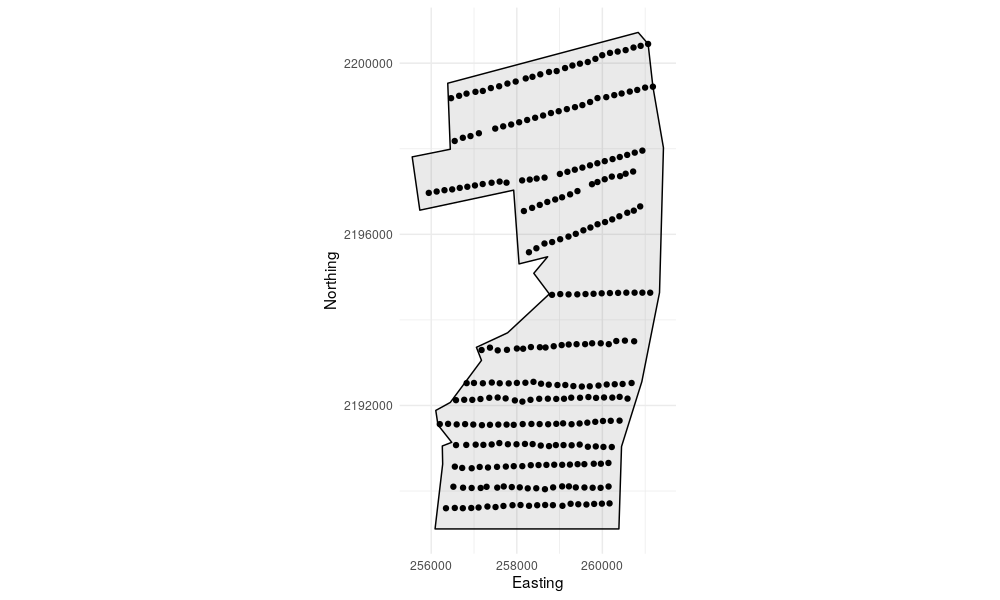
\includegraphics[scale=0.5]{figures/study_area_design.png}
	\caption{Study area showing the 2002 survey points (black dots) in Hakalau Forest National Wildlife Refuge, \hawaii{} Island.}
	\label{fig:2002studyareapointspt}
\end{figure}

Surveys used point-transect methods, recording horizontal distances from survey points to individually detected birds. Surveys commenced at dawn and continued until 11:00 or halted when weather conditions exceeded prescribed conditions that hindered detecting birds (light rain, and wind and gust strength \textgreater Baufort scale 3). During 8-min counts trained observers recorded the species, exact distance to the nearest meter and detection type for each bird detected, along with the sampling conditions cloud cover, rain, wind strength, gust strength, and time of day each point was surveyed.  \cite{camp_population_2010,camp_statespace_2016} provide a detailed description of Hakalau, the study area and the bird surveys.

For the purposes of our analysis we select a single survey year from the \akepa{} time series that contained on broad sampling of the study area with sufficient numbers of detections to estimate detectability. In 2002, 289 points were sampled using point-transect distance sampling methods within the 4,603 ha study area of Hakalau (Fig. \ref{fig:2002studyareapointspt}) during which 276 \akepa{} were detected on 121 point transects. The number of detections within each point transect ranged from zero to six. We select a single year of data to demonstrate our approach in a simplified setting where temporal aspects of analysis are not considered.  Our approach is easily extendible to spatio-temporal modelling frameworks which we discuss in more detail in the discussion.

\section{Distance sampling as a thinned point process}

\subsection{Overview of distance sampling methods}

Distance sampling methods aim to estimate abundance by using a spatially explicit sampling design and an assumed detection model to estimate the detectability of animals as a function of distance from transect \citep{buckland_advanced_2004, buckland_distance_2015}.  Classic distance sampling approaches use a hybrid of design- and model-based inference to estimate population size where the probability of detection is modelled and a randomized sampling design allows the construction of Horvitz-Thompson-like estimators of animal density \citep{horvitz_generalization_1952,  buckland_advanced_2004}.

More recently, interest has focused on fully model-based approaches that include a spatially explicit model for animal density and allow non-randomized survey designs to be used.  These methods allow density to be associated with spatially-indexed covariates and animal density can, in principle, be estimated or predicted for any subregion within the study area \citep{johnson_model-based_2010, miller_spatial_2013, buckland_model-based_2016}.  This additional flexibility to make predictions for smaller, user-specified geographic units, has made model-based distance sampling a common approach in the literature \citep{garciabaron_modelling_2019, herr_aerial_2019, breen_new_2017, williams_chilean_2011, stokes_monitoring_2010, williams_modeling_2006}.

Model-based distance sampling has most commonly been implemented in a two-stage modelling framework, see the \texttt{dsm} package \citep{miller_spatial_2013}, for example.  In the first stage, detectability is estimated.  In the second stage, detectability estimates from the first stage are used as an offset in a generalized additive model framework.  Detections within sampling units are binned into counts and an appropriate response distribution is chosen.  Due to the often sparse nature of wildlife survey data this may require consideration of over- or under-dispersion and zero-inflated distributions.  Negative-binomial and Tweedie distributions are common choices.  This two-stage approach has come under the name \textit{density surface models} and \cite{miller_spatial_2013} provide a review.

A key concern with the two-stage approach is the propagation of uncertainty from the detection model to the second-stage spatial model.  Early attempts to address this focused on bootstrapping \citep{lahiri_resampling_2003, hedley_spatial_2004} but more recent work has pointed to potential difficulties of the bootstrapping approach, noting the difficulty of choosing the resampling units when combining spatially structured random effects and spatial bootstraps \citep{bravington_reliable_2018-1, williams_chilean_2011}. Instead, \cite{bravington_reliable_2018-1} propose avoiding bootstrapping by propagating error based on a second-order Taylor approximation of detectability around the first-stage maximum-likelihood estimate.

Concerns about uncertainty propagation can be avoided by using one-stage modelling approaches.  These approaches tend to be Bayesian and use data augmentation to model unobserved individuals or groups and Markov-chain Monte Carlo (MCMC) methods for inference \citep{royle_hierarchical_2008, schmidt_using_2012}.  \citet{oedekoven_bayesian_2014} demonstrate a one-stage model that avoids data augmentation by specifying a combined likelihood of the detection and spatially-explicit count models and incorporated model uncertainty using reversible jump MCMC.  

The only Bayesian one-stage analysis that does not use MCMC is, to the best of our knowledge, \citet{yuan_point_2017}, who use the approximate Bayesian method of integrated nested Laplace approximations (INLA) \citep{rue_approximate_2009} applied to line transect distance sampling data.  INLA is a popular choice for fitting models with spatially-structured random effects in large or complex spatial domains due to the implementation of a computationally efficient approach based on the construction of a sparse prior precision matrix for the random effect parameters.  This sparse precision matrix specifies a GMRF representation of a Gaussian random field defined as the stationary solutions to an SPDE \citep{lindgren_explicit_2011} (see Section \ref{GMRFexplanation} for more details on this approach).  The finite element methods involved use a flexible triangulation of the spatial domain and have been shown to be more efficient than regular lattice based approaches \citep{simpson_going_2016}, a useful feature for applications with complex boundaries which appear in wildlife survey data such as boundaries formed by coastlines, rivers and other natural features. 

\citet{yuan_point_2017} also take a point process perspective and formulate the detection model as a thinning of the full, but imperfectly observed, point pattern.  Key to their approach was formulating the detection model as the solution to an SPDE.  Choosing a B-spline basis and applying finite element methods results in a sparse prior precision matrix for the detection model coefficients which can then be incorporated into INLA using the same machinery as already exists for latent Gaussian precision matrices.  A major downside to this approach is that the solutions to the detection model SPDE are not necessarily monotonically decreasing - usually a key feature of detection functions.  The authors' suggestion to reject any non-monotonically decreasing functions when sampling from the posterior is potentially computationally wasteful. 

Here we present a related approach to the one in \citet{yuan_point_2017} in that our models are fitted using INLA.  However, we avoid these issues with the SPDE detection model, instead allowing the user to specify a parametric family of detection functions, such as the half-normal, as a user-written R function.  This approach of choosing a parametric family of detection functions will be more familiar to users of classical distance sampling methods than the SPDE specification.  However, this parametric form results in components of the additive predictor that are non-linear in their parameters, making model fitting infeasible in the \text{R-INLA} \citep{rue_approximate_2009} package implementation of INLA.  We address this by using a method of iterated model fits based on a Taylor expansion of the non-linear model components and implemented in the \texttt{inlabru} package \citep{bachl_inlabru_2019}.

We apply these methods to point transect \akepa data which differ from line transect methods to account for the fact that the area surveyed increases with increasing distance from the transect.  Our analysis is, to the best of our knowledge, the first analysis of point transect distance sampling data formulated as a thinned point process.  However, the point process viewpoint is not new and has been taken numerous times in analyses of line transect data \citep{buckland_model-based_2016, niemi_bayesian_2010, johnson_model-based_2010, waagepetersen_likelihood-based_2006, hedley_spatial_2004,  hogmander_random_1991, stoyan_remark_1982}.  

\subsection{Model specification}

In this section we introduce the statistical model for the spatial pattern of animal locations and the observation process, including a detailed description of how this model can be written as a modified Poisson likelihood.  We use this formulation to fit the model using the software package \texttt{inlabru} \citep{bachl_inlabru_2019}, an extension to the \texttt{R-INLA} implementation of INLA, which implements the iterated INLA approach and is available through the Comprehensive R Archive Network \citep{r_2017}.

We assume the location of animals are a point pattern that follows a log-Gaussian Cox process with intensity process $\lambda(.)$, i.e.  the intensity at location $s$ is a random variable $\lambda(s)$.  The log-Gaussian Cox process is a flexible approach that can include spatial covariates to model the mean intensity and a mean-zero spatially structured random effect to account for unexplained heterogeneity not captured by the covariates \citep{moller_log_1998}.

To account for the imperfect detection of points we specify a thinning probability function $g(s) = \mathbb{P}(\text{a point at $s$ is detected | a point is at $s$})$. A key property of the log-Gaussian Cox process is that a realisation of a point process with intensity process $\lambda(s)$ that is thinned by thinning probability function $g(s)$ also follows a log-Gaussian Cox process with intensity given by $\tl(s) = \lambda(s)g(s)$.

Standard distance sampling approaches specify $g(s)$ as a function that decays with increasing distance.  The type of distance measured depends on the type of survey.  For line transects the perpendicular distance to the transect line is used.  For point transects the horizontal distance to the observer is the relevant distance.  For the remainder of the paper we assume a point transect survey design and hence horizontal distance to the observer located at the centre of the point transect.  

The thinning probability function is specified as a parametric family of functions with parameter vector.  For example, if $r(s)$ denotes the distance of a point at $s$ from the observer, the half-normal thinning probability function is $g(s | \sigma) = \exp(-r(s)^2 / 2\sigma^2)$, where $\sigma^2 > 0$ is a variance parameter to be estimated.  Other types of detection function exist, such as hazard-rate, negative exponential, and they may or may not be adjusted using series expansions to add some flexibility to obtain a better fit to a given dataset \citep{buckland_distance_2015}.  In this analysis we assume a half-normal detection function with no covariates on detection parameters.

The detection function parameters can only be estimated if an assumption is made about the intensity of the animal locations.  Without such an assumption detectability and intensity are confounded.  The standard assumption in distance sampling is that the intensity is constant with respect to changes in $r(s)$.  Thus any observed deviations from uniformity can be attributed to detectability and not to variation in the intensity.

A point transect distance sampling survey consists of a set of $K$ point transects.   We denote $k$-th subset of space covered by the $k-th$ point transect as $\Omega_k \subset \mathbb{R}^2$ and the total surveyed region is $\Omega = \cup_{k=1}^K \Omega_k$.  For simplicity, we assume that all point transects are non-overlapping discs with radius $W$, as is the case in the HFBS survey.  The probability of observing a point at location $s \in \Omega_k$ given it is at $s \in \Omega_k$ we denote $g_k(s)$.  The probability of observing a point outside the surveyed region is zero.
Since the point transects are non-overlapping, each location $s \in \Omega$ is unambigiously associated with a single thinning probability function $g_k$.  For example, for an observer at location $s_k \in \Omega_k$, the centre of the disc, the half-normal thinning probability function is $g_k(s) = \exp(-\lVert s - s_k \rVert_2^2 / 2\sigma^2)$.  In practice the observer is always located at the centre of the point transect.  The assumption of non-overlapping survey regions could be relaxed by including extra information such as the time of each observation but this is not a requirement here.  The thinning probability function for any $s \in \Omega$ is then given by $g(s) = g_{k(s)}(s)$ where $k(s) = k$ for $s \in \Omega_k$.

The thinned log-Gaussian Cox process likelihood with observed points at locations $\bm{Y} = (s_1, \ldots, s_n)^\intercal$ is then
\begin{equation}
\label{lgcp-likelihood}
\pi(\bm{Y}) = \exp\left( |\Omega| -\int\displaylimits_{s \in \Omega} \lambda(s) g(s) \mathrm{d}s \right)\prod_{i=1}^n \lambda(s_i)g(s_i)
\end{equation}
where $\lambda(.)$ and $g(.)$ both depend on parameter vectors omitted for readability and $|\Omega|$ is the area of the total surveyed region.  

\subsection{Writing the model as a modified Poisson likelihood}

\sloppy Here we show how to approximate the thinned log Gaussian Cox process model with a modified Poisson likelihood.  The integral component $\int\displaylimits_{s \in \Omega} \lambda(s) g(s) \mathrm{d}s$ in \autoref{lgcp-likelihood} does not have analytical solutions.  Replacing the integral with a weighted sum allows the log-likelihood to be approximated as a weighted Poisson log-likelihood, which we describe below, adapting the approach developed by \cite{simpson_going_2016} for a fully observed point pattern.

To evaluate the integral we use polar coordinates notation $s_k(r, \theta) = s_k + r\left[\cos\theta, \sin\theta \right]^T$ to represent locations in each sampling unit $\Omega_k$.   In general, the thinning function depends only on $r$ and not on $\theta$.  We assume this is the case in the following and use the shorthand $g_k(r) = g(s_k(r, \theta))$. The integral in the likelihood can be simplified using an assumption that $\lambda(s)$ is linear within each sampling unit.  This assumption implies that $\lambda(s_k(r, \theta)) + \lambda(s_k(r, \theta + \pi)) = 2\lambda(s_k)$ and so
\begin{align*}
	\int_0^{2\pi} \lambda(s_k(r, \theta))g_k(r)\mathrm{d}\theta &= \int_0^\pi \left[\lambda(s_k(r, \theta)) + \lambda(s_k(r, \theta + \pi)) \right] g_k(r)\mathrm{d}\theta \\
	&= 2\pi \lambda(s_k)g_k(r)
\end{align*}
We note that this is a relaxation of the traditional assumption in distance sampling that the intensity is constant within each sampling unit.  A similar relaxation is also possible in the case of line transects \citep{yuan_point_2017} and this assumption complements the choice of piece-wise linear basis functions we use to model $\lambda$ (see section 5).  Integrating with respect to $r$ and accounting for the change of variables gives $\int \lambda(s)g(s) \mathrm{d}s = \sum_{k=1}^K 2\pi \lambda(s_k) \int_0^W r g_k(r)\mathrm{d}r$.   For each sampling unit we approximate the one-dimensional integral with respect to $r$ using a midpoint integration method with $M$ integration locations $r_{k1}, \ldots, r_{kM}$ and associated weights $\alpha_{k1}, \ldots, \alpha_{kM}$.  This gives
\begin{equation*}
	\int\displaylimits_{s \in \Omega} \lambda(s)g(s)\mathrm{d}s \approx \sum_{k=1}^K \sum_{j=1}^M \tilde{\alpha}_{kj} \tl(s_{kj}) \;\;\; ,
\end{equation*}
where $\tilde{\alpha}_{kj} = 2\pi \alpha_{kj}r_{kj}$ and $\tl(s_{kj}) = \lambda(s_k) g_k(r_{kj})$.

To simplify notation below we let $\tilde{\alpha}_{k} = (\alpha_{k1}, \ldots, \alpha_{kM})^\intercal$ and $\tilde{\alpha} = (\alpha_1^\intercal, \ldots, \alpha_K^\intercal)^\intercal$.  Similarly, let $\tl_k = (\tl(s_{k1}), \ldots, \tl(s_{kM}))^\intercal$, $\tl_{int} = (\tl_1^\intercal, \ldots, \tl_K^\intercal)^\intercal$ and denote the intensity evaluated at the observed locations as $\tl_{obs} = (\tl(s_1), \ldots, \tl(s_n))^\intercal$.  Then the approximate log-likelihood is
\begin{equation}
\label{approx-log-likelihood}
	\log \pi(\bm{Y}) \approx - \tilde{\alpha}^\intercal \tl_{int} + 1^\intercal\log\tl_{obs}
\end{equation}
This approximation can be expressed as a modified Poisson likelihood.  To see this let $\eta = (\tl_{int}^\intercal, \tl_{obs}^\intercal)^\intercal$,
$\alpha = (\tilde{\alpha}^\intercal, 0_{n \times 1}^\intercal)^\intercal$ and construct a vector of pseudo-observations $z = (0_{KM\times 1}^\intercal, 1_{n \times 1}^\intercal)^\intercal$.  Then the approximate likelihood becomes
\begin{equation}
\pi(\bm{Y}) \approx C \prod\limits_{i=1}^{KM + n} \eta_i^{z_i}\exp(-\alpha_i\eta_i)
\end{equation}
where $C$ is a constant.  This approximate likelihood is implemented in \texttt{inlabru} as a \texttt{"cp"} likelihood.  This is similar to the Berman-Turner device \citep{berman_approximating_1992, baddeley_practical_2000} although without the assumption that the locations of observed points form a part of the quadrature scheme.

\subsection{Intensities for incomplete data}

In the above, we assume the data are complete records of animal locations.  However, in many distance sampling surveys only the location of the observer and the distance to the observer are recorded.  Data of this type can be analysed within a point process framework by deriving the appropriate intensity function for the incomplete data as outlined below.

Using the polar coordinates notation given above, for a detected point at location $s_k(r, \theta) \in \Omega_k$ we consider the case where we observe $r$ but not $\theta$.  It follows that the intensity for points at a distance $r$ observed within sampling unit $\Omega_k$ is
\begin{align}
\label{intensity-incomplete}
\tl_k(r) &= \oint\displaylimits_{c_k(r)} \lambda(s)g_k(r)\mathrm{d}s \nonumber \\
&= 2\pi\lambda(s_k)rg_k(r) \;\;\; ,
\end{align}
 where $c_k(r)$ is a circle of radius $r$ centred at $s_k$ and the second line follows from changing to polar coordinates and the assumption of linear intensity within $\Omega_k$.  This intensity differs from the full data case through the $2\pi$  term that accounts for the fact that we do not observe $\theta$ and the additional $r$ term that accounts for the increasing area surveyed at larger distances.  The log-intensity for observed points (the thinned intensity) is thus $\log\tl(s) = \log 2 \pi r + \log\lambda(s) + \log g(s)$ and so can be implemented during fitting by using an offset.  As we noted above, the detection function $g(s)$ is non-linear in its parameters and this component of the additive predictor requires a novel approach to parameter estimation.

\section{Iterated INLA}

The half-normal detection function depends on the strictly positive parameter $\sigma^2$.  We choose a log link and consider $g(s | \phi)$, where $\log\sigma^2 = \phi$.  However, this model cannot be directly fitted using INLA since $\log g(s | \phi)$ is not linear in its parameters.  To address this we use an approximate method based on a first-order Taylor approximation of the non-linear predictor.  Let $\eta(\bm{u}) = \log \tilde{\lambda}(\bm{u})$ where $\bm{u}$ is the parameter vector of the predictor (which includes $\phi$ as well as any parameters for fixed and random effects).  Denote by $\bar{\eta}_{\bm{u}_0}$ the first-order Taylor approximation of $\eta(\bm{u})$ at the point $\bm{u}_0$.  That is
\begin{equation*}
\bar{\eta}_{\bm{u}_0} = \eta(\bm{u_0}) + \bm{B}_{\bm{u}_0}(\bm{u} - \bm{u}_0)
\end{equation*}
where $\bm{B}_{\bm{u}_0}$ is the derivative matrix of $\eta(\bm{u})$ evaluated at $\bm{u}_0$.  Since $\bar{\eta}_{\bm{u}_0}$ is linear in $\bm{u}$ it is possible to fit an approximate model in INLA by replacing the non-linear $\eta$ with the linear Taylor approximation $\bar{\eta}_{\bm{u_0}}$.   The question then is how to choose the linearisation point $\bm{u}_0$.  The approach taken is via a fixed point iteration scheme.  There are many possible choices here and we describe the approach in the current implementation of \texttt{inlabru} \citep{bachl_inlabru_2019}.  However, more options are likely to be added in the future.  We denote by $\bar{p}_{\bm{v}}$ the posterior distribution of the model parameters given the linearised model configuration at linearisation point $\bm{v}$ and define the functional
\begin{equation}
	f(\bar{p}_{\bm{v}}) = \left\{ \argmax_{\bm{u}_i} \: \bar{p}_{\bm{v}}(u_i | \bm{Y}), \quad i = 1, \ldots, n_{\bm{u}} \right\}
\end{equation}  
where $n_{\bm{u}}$ is the length of $\bm{u}$.  Each $\bar{p}_{\bm{v}} (u_i | \bm{Y})$ is approximated and the mode estimated during the model fitting using the standard INLA method.
We then seek a fixed point of this functional so that $\bm{u}_0 = f(\bar{p}_{\bm{u}_0})$.  This fixed point is identified via an iterative scheme.  Given a current choice of linearisation point $\bm{v}$, estimate $\bar{p}_{\bm{v}}$ and set $\bm{u}_* :=f(\bar{p}_v)$ to use as the new linearisation point.  Iterate this procedure until a fixed point is identified within a chosen tolerance.  

In practice the point $\bm{u}_*$ may be problematic and result in a linearised model configuration that is challenging to fit.  Instead this point is considered only as an initial candidate point.  The next linearisation point is chosen by setting $\bm{u}_{\alpha} = (1 - \alpha)\bm{v} + \alpha \bm{u}_*$ and finding the value of $\alpha$ that minimises $ \lVert \eta(\bm{u}_{\alpha}) - \bar{\eta}_{\bm{v}} \rVert$.  This means that the new linearisation point remains close to a feasible region for fitting, assuming the current point $\bm{v}$ is reasonable.  We estimate $\alpha$ using an approximate line search method that avoids many potentially expensive evaluations of the non-linear predictor.  This iterative method is implemented in the R package \texttt{inlabru} \citep{bachl_inlabru_2019}.

\section{Spatially Structured Random Effect}
\label{GMRFexplanation}

Using spatially-structured random effects can be computationally expensive, often resulting in dense prior precision matrices which typically have $\mathcal{O}(n^3)$ cost to factorise for an effect with $n$ parameters.  A key development in this area is the use of sparse Gaussian Markov random field (GMRF) representations of Gaussian random fields (GRFs) and the \texttt{R-INLA} software that makes use of the sparsity to factorise the precision matrix at a cost of $\mathcal{O}(n^{3/2})$.  This representation is constructed via a stochastic partial differential equation solved using finite element methods \citep{lindgren_explicit_2011}.

The log-intensity of animal locations is given by
\begin{equation*}
\log \lambda(s) = \beta_0 + \sum_v \beta_v z_v(s) + \xi(s)
\end{equation*}
where $\beta_0$ is an intercept parameter, the $z_v(s)$ are spatial covariates with effect parameters $\beta_v$ and $\xi(s)$ is a zero-mean GRF with Mat\'ern covariance
\begin{equation}
C(s_1,s_2) = \frac{2^{1-\nu}}{4\pi\kappa^2\tau^2\Gamma(\nu)}(\kappa \|s_1-s_2\|)^{\nu}K_\nu(\kappa \|s_1-s_2\|)
\end{equation}
where \(\nu, \kappa, \tau\) are parameters and \(K_{\nu}\) is the modified Bessel function of the second kind.  All three parameters are not simultaneously identifiable \citep{zhang_inconsistent_2004} and it is conventional to assume a value for $\nu$ which specifies the mean-square differentiability of the process.  We set $\nu = 1$ which is the default value in \texttt{R-INLA}.

We use a GMRF representation of $\xi(s)$ following the approach of \cite{lindgren_explicit_2011} based on specifying $\xi(s)$ via a SPDE.  Given a finite element mesh on the spatial domain with $L$ nodes and associated piece-wise linear basis functions $\phi_1, \ldots, \phi_L$ we represent the GRF as $\xi(s) = \sum_l \xi_l \phi_l(s)$.  The parameters $\xi_1, \ldots, \xi_L$ form a GMRF with sparse prior precision matrix $\bm{Q}_{\xi} = \frac{1}{\tau^2}\left(\kappa^4\bm{C} + 2\kappa^2\bm{G_1} + \bm{G_2}\right)$ where $\bm{C}$, $\bm{G_1}$, $\bm{G_2}$ are all sparse matrices the elements of which are defined via an approximate solution to a SPDE (see Supplementary material). The parameters $\tau$ and $\kappa$ control the shape and rate of decay of the Mat\'ern covariance function. In order to specify priors on the Mat\'ern covariance below we use a reparameterisation to a range and variance parameter.  When $\nu = 1$ and the domain is of dimension two the reparameterisation is $\rho = \sqrt{8} / \kappa$ and $\sigma^2 = 1 / (4\pi\kappa^2\tau^2)$ \citep{blangiardo_spatial_2013}.  

The SPDE approach can at first appear to be fundamentally different to other spatial random effect approaches such as penalised regression splines.  However, the two methods are closely related and the GRF model component in our model plays a similar role to a tensor product spline with an appropriate smoothing penalty.  See \cite{yue_bayesian_2014, miller_understanding_2019} for more details on the similarities and differences between penalised regression splines and the SPDE approach.  

\section{Results}
\label{results}

We fitted the models using penalised complexity priors for the hyperparameters of the GMRF \citep{simpson_penalising_2017}, setting $\mathbb{P}(\sigma > 2) = 0.01$ and $\mathbb{P}(\rho < 130) = 0.01$, where $\rho$ is the range parameter of the Mat\'ern covariance.  The value of 130 was selected based on the minimum distance between sampling locations.  The complete code for the analysis can be found in the Supplementary materials.  Since only distance to observer was recorded we used the adjusted intensity given in \eqref{intensity-incomplete}.   

The predicted mean of the posterior intensity is shown in \autoref{fig:intensity-mean-cv} along with a map of the coefficient of variation (CV) of the posterior intensity field on a regular prediction grid with cell area of approximately 1.7 hectares.  
\begin{figure}[h]
	\begin{center}
		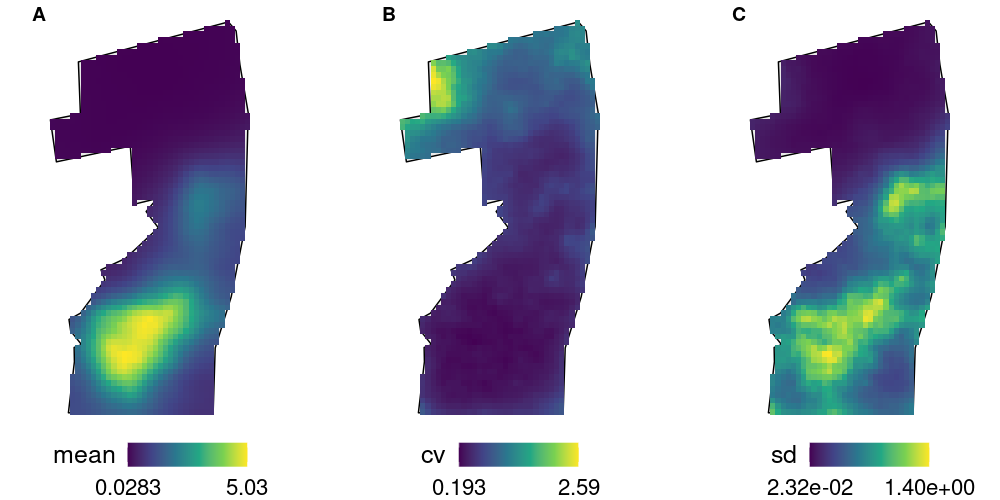
\includegraphics[scale=0.525]{figures/intensity_mean_cv_sd.png}
		\caption{The A) mean, B) CV and C) SD of the posterior intensity field.  Units are per m$^2$}
		\label{fig:intensity-mean-cv}
	\end{center}
\end{figure}
This shows a region of high intensity in the south and much lower intensity in the north, agreeing with a standard two-stage analysis of the same data (see Supplementary material).  The CV plot shows that the CV in the posterior intensity field is lower in areas with greater sampling effort.  There is a clear indication of preferential sampling with more survey effort in the south, where densities are higher, compared to the north  (see \autoref{fig:2002studyareapointspt}).  In the north, estimated intensities are lower, which also contributes to larger CV values.  The standard deviation map shows stronger overall posterior variability in the south where intensity is larger.  We also map the lower and upper quantiles corresponding to a 95\% credible interval for each prediction location.  [[Say something about these - hard to know what to say about them?]]   (\autoref{fig:intensity-quantiles}).
\begin{figure}[h]
	\begin{center}
		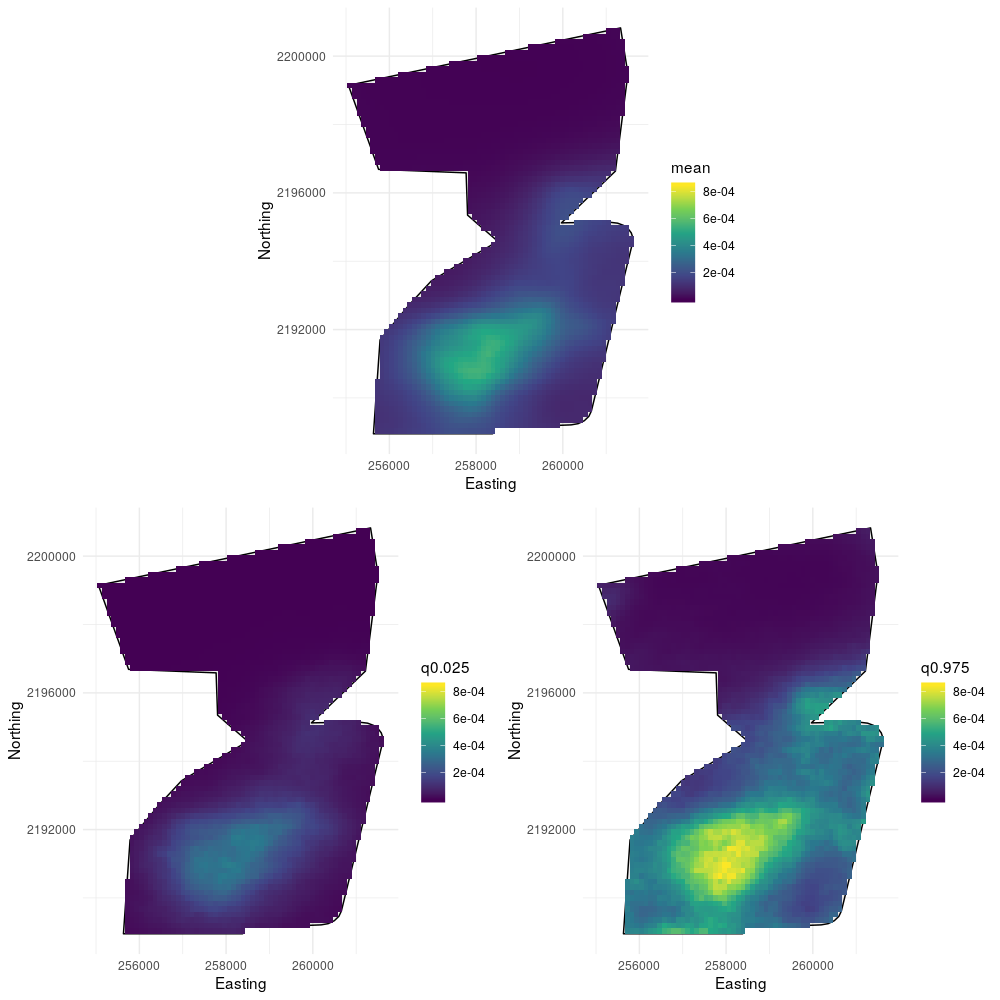
\includegraphics[scale=0.525]{figures/intensity_quantiles.png}
		\caption{The predicted posterior intensity quantiles:  A) 0.025 quantile B) 0.975 quantile.  Both plots plots use the same colour scale}
		\label{fig:intensity-quantiles}
	\end{center}
\end{figure}

The posterior detection function \autoref{fig:det-matern} shows that detectability drops to just under 0.25 at the maximum observable distance of 58 metres.
\begin{figure}[h]
	\begin{center}
		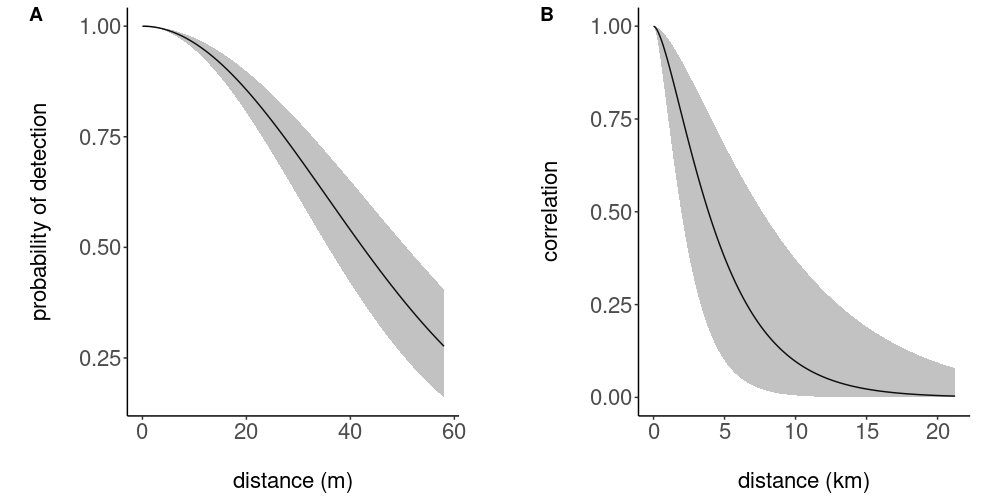
\includegraphics[scale=0.525]{figures/detfn_and_matern.png}
		\caption{A) posterior half-normal detection function. B) posterior Mat\'ern correlation function.  The black line is the mean posterior estimate and the grey shaded area is 95\% credible interval in both plots}
		\label{fig:det-matern}
	\end{center}
\end{figure}
The posterior Mat\'ern correlation function is shown in \autoref{fig:det-matern}, the grey regions show the 95\% credible interval.  Note that this correlation function shows positive correlation even at distances of 10,000 metres, wider than the full length of the study region (approximately 8,000 metres).  This is the correlation range on the log-intensity scale.  [[Can I make a better "range of correlation" plot for the posterior intensity process?  How can I convert this to something on the intensity scale?  For a field $Z$ with covariance function $C$, is there an implied covariance for $\exp(Z)$?]]

To further investigate the ability of the GMRF component to capture the heterogeneity we generated 100 thinned point patterns from the fitted model and calculated the pairwise distances between all observations for each of these patterns \autoref{fig:post-pp-distances}.  
\begin{figure}[h]
	\begin{center}
		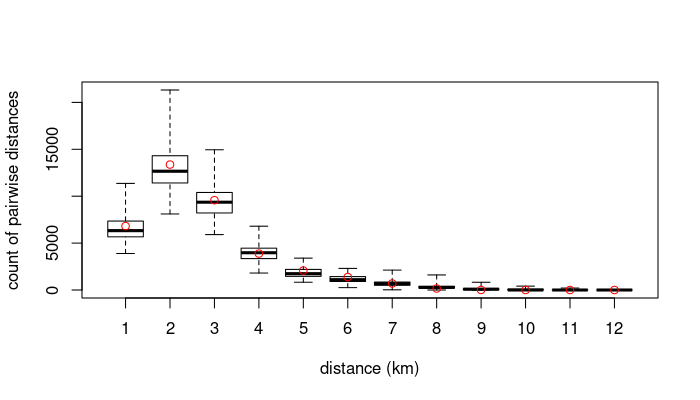
\includegraphics[scale=0.6]{figures/post_pp_distances.png}
		\caption{Boxplots of frequency of pairwise distances (tick mark values for end of each bin) based on 100 posterior samples.  Red circles: observed frequency of pairwise distances between observations}
		\label{fig:post-pp-distances}
	\end{center}
\end{figure}
The plot shows that the GMRF component broadly captures the relevant scale of clustering in the observed data.  There is some evidence of over-predicting the strength of the clustering at distances between 1,000 and 2,500 m.  

We plot the posterior abundance estimate using a Monte Carlo method.
\begin{figure}[h]
	\begin{center}
		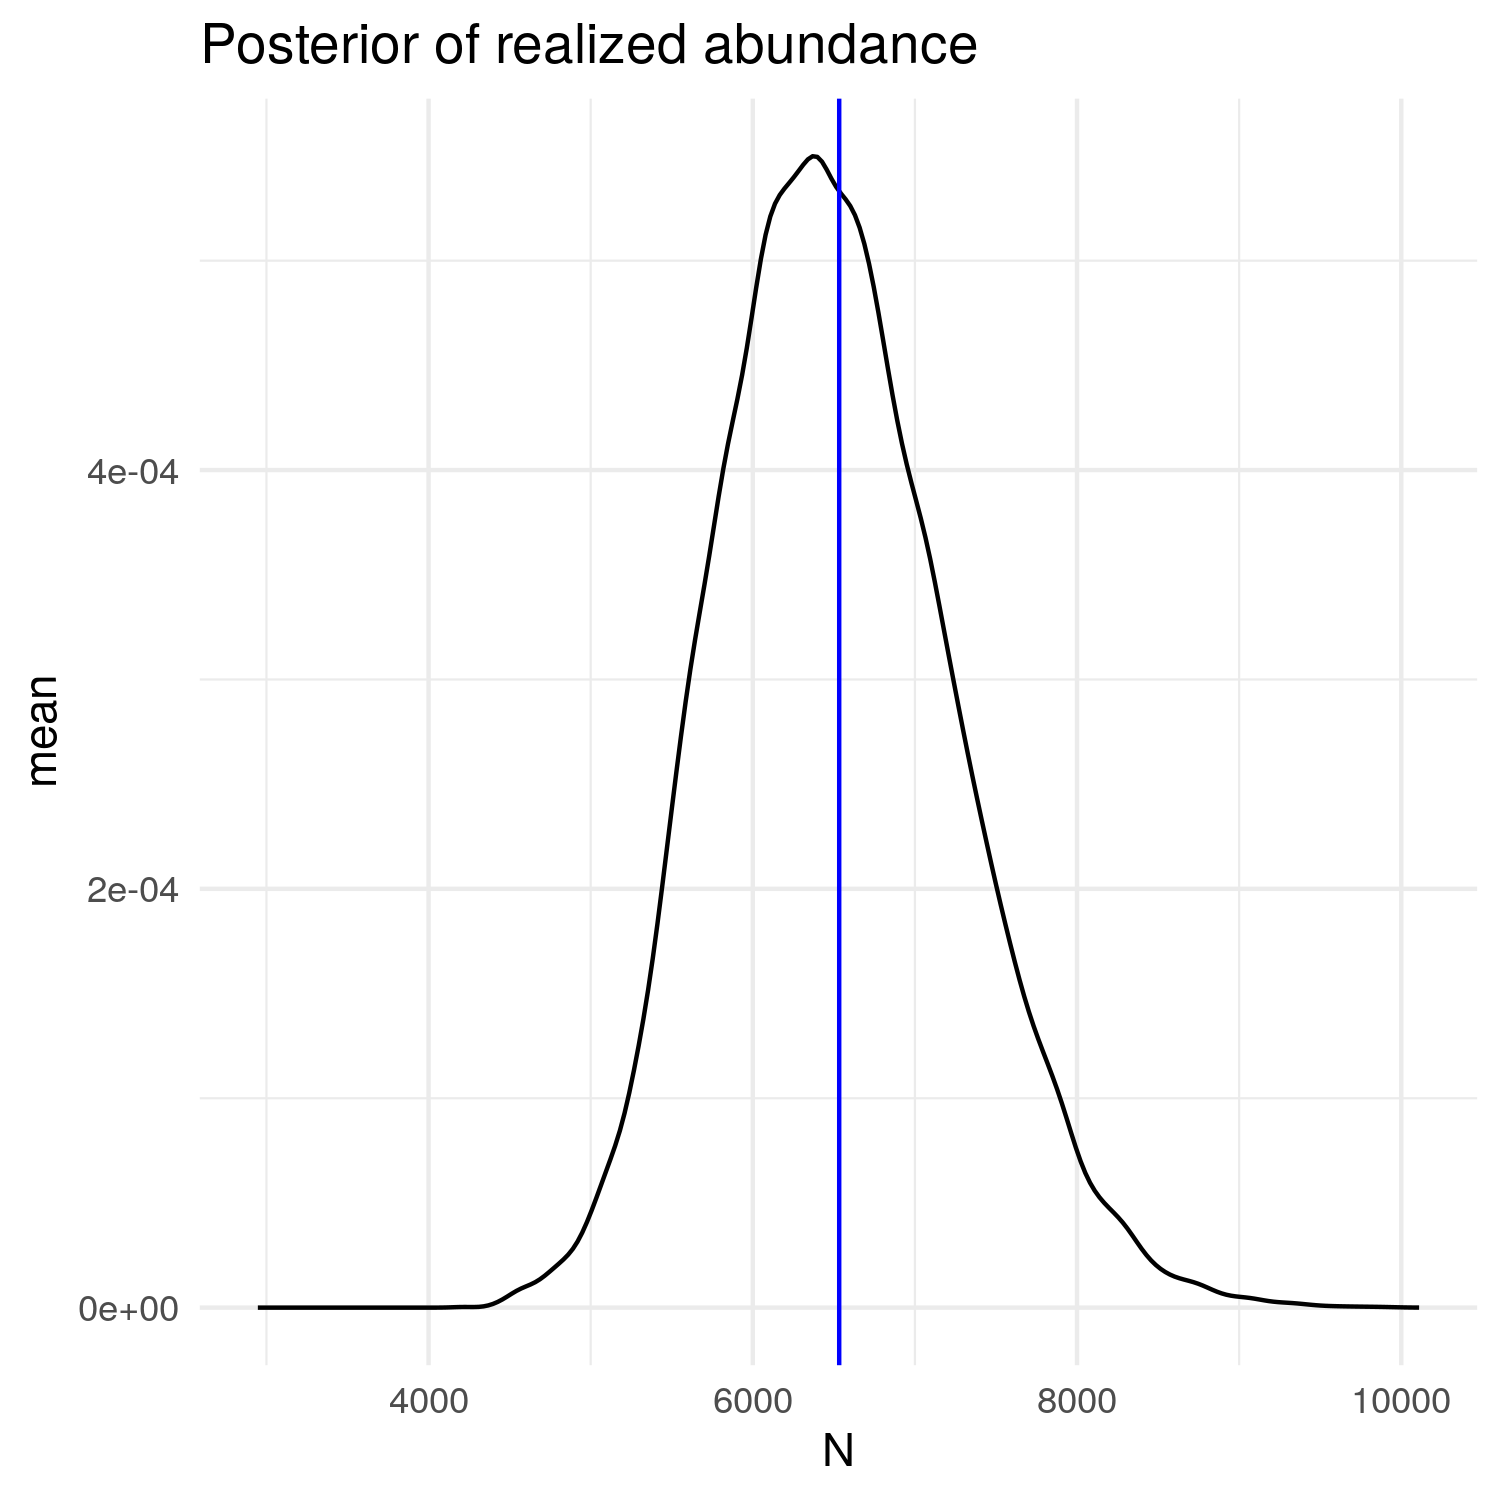
\includegraphics[scale=0.525]{figures/realized_abundance_posterior.png}
		\caption{Posterior abundance}
		\label{fig:realized-abundance-posterior}
	\end{center}
\end{figure}
Let $n$ denote the abundance of the population within the region of interest and $N = \int_{\Omega}\lambda(s)\mathrm{d}s$ its corresponding random variable within our Bayesian framework.  Integrating the mean of the posterior intensity field provides a point estimate for the abundance, i.e. the expected abundance.  We approximate the posterior $\pi(N | \bm{Y})$ by a Monte Carlo method.  Taking $m$ Monte Carlo samples  $\lambda^{(1)}, \ldots, \lambda^{(m)}$ of the posterior intensity field we estimate the posterior for the abundance as $\pi(N | \bm{Y}) \approx 1 / m \sum_{i=1}^m \pi (N | \lambda = \lambda^{(i)})$. Each $\pi(N | \lambda = \lambda_i)$ is a Poisson probability mass function with rate parameter $\int_{\Omega}\lambda_i(s)\mathrm{d}s$. \autoref{fig:realized-abundance-posterior} shows the approximate posterior for $N$ with $m = 20,000$.  This allows us to estimate the probability for any specific value of realised abundance $n$ by estimated $\pi(N = n | \lambda)$.  Strictly speaking 
  
% Add table of estimated model parameters
% Add 95% CI figures for N?

\clearpage %sort out figure placements later

\section{Communication of Results}

The results above are consistent with those resulting from a two-stage model fitted to binned count data (see Supplementary material).  Our presentation of the results is broadly consistent with approaches taken in the species distribution modelling literature, although maps of predictive uncertainty (\autoref{fig:intensity-mean-cv} and \autoref{fig:intensity-quantiles}) are not always provided there and it is common to see maps of point estimates without any accompanying communication of uncertainty.  It is also common to report a point estimate of the expected abundance along with uncertainty in this point estimate.  However, uncertainty in a point estimate will tend to have lower variance than variance of the random variable of interest.  For this reason we chose to show the full abundance posterior in \autoref{fig:realized-abundance-posterior}.

Our intention in this section is to highlight limitations with mapped summaries of model predictions, including those presented in Section \ref{results}, and suggest ways to address these limitations.  We note that all model outputs are based on sampling from the joint posterior of all model parameters which naturally average over the uncertainty in the observation process, a key advantage of the one-stage approach.   

\subsection{Limitations of mapped summaries}

The mapped posterior mean is the most common map one encounters in the literature.  However, the mean will always be smoother than realisations from the posterior random field.
\begin{figure}
	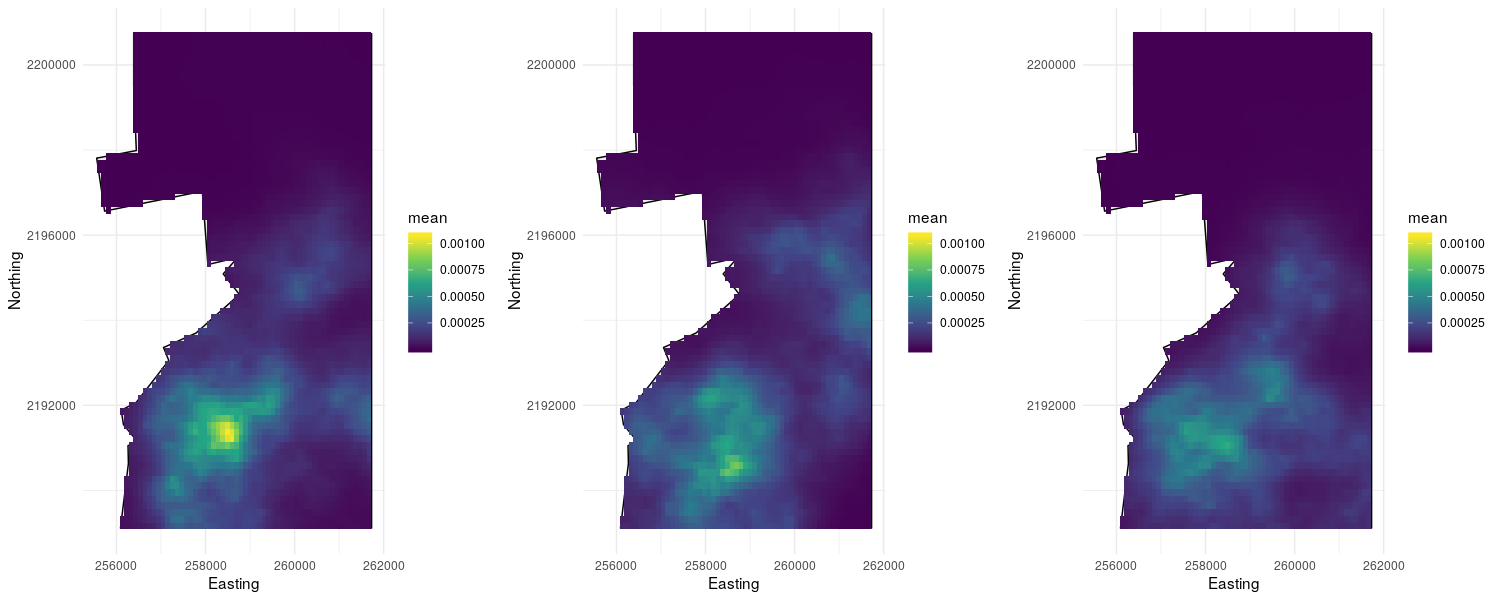
\includegraphics[scale=0.525]{figures/intensity_realized.png}
	\caption{Three realizations of the posterior intensity field}
	\label{fig:intensity-realizations}
\end{figure}  
\autoref{fig:intensity-realizations} shows three such realisations from the posterior intensity field.  Note that each realisation has a finer-grained spatial structure than is shown in the posterior mean (\autoref{fig:intensity-mean-cv}A).  Hence, considering this finer-grained structure, our interpretation is that the clustering of animals is stronger than might be expected if we only looked at the posterior mean.  Similarly for model evaluation we recommend plotting multiple realisations of the posterior field as these will more closely resemble the spatial structure of the observed data.  Noting differences between realisations is also an effective way to communicate uncertainty.

The CV map (\autoref{fig:intensity-mean-cv}B) is also intended to communicate uncertainty.  However, CV values will be higher in regions of low predicted intensity, particularly if the posterior standard deviation is relatively consistent across the study region or positively correlated with the intensity.  The observed patterns in such maps will highlight regions of relatively lower intensity, not necessarily higher overall uncertainty.  This is clearly the case in \autoref{fig:intensity-mean-cv}B.  

The standard deviation map (\autoref{fig:intensity-mean-cv}C) does show clearly the spatially varying uncertainty.  However,  care should be given to what the mapped values imply in the context of a given analysis.  A default colour scale will nearly always show some spatial variation in uncertainty, with some regions of relatively high or low uncertainty.  What such a map does not show is whether these differences actually matter in the context of the analysis.  For example, it could be the case that the standard deviation values are so large as to make the predictions have an unacceptably high uncertainty everywhere.  Or, on the other hand, perhaps differences between high and low uncertainty regions (`high' and `low' as defined by the default colour scale) are small enough to be negligible when it comes to making conclusions or decisions, in which case such a spatially varying map is not a relevant output of the analysis.  These are two extreme examples.  However, cases in between suffer from the same problem.  

The quantile maps also suffer from a potential difficulty in interpretation. The temptation is to perceive the maps as showing possible intensity surfaces that could have produced the observed data.  However, presenting these quantiles together in a single map obscures the fact that it is vanishingly unlikely for all prediction values to simultaneously achieve the 0.025 or 0.975 quantile.  A similar problem will occur if mapping the marginal probability of exceeding a threshold at each prediction location.  We believe these caveats make the map difficult to use for most non-statistically trained audiences.  To demonstrate the possible consequences of this we (incorrectly) treat the lower and upper quantile plots as though they were intensities and integrated them to obtain an expected abundance estimate of approximately 3,300 for the 0.025 quantile map and 12,400 for the 0.975 quantile map.  A naive (and tempting) interpretation of these numbers is as lower and upper limits of the 95\% credible interval for abundance. However, these abundance estimates are outside the support of the posterior for abundance (see \autoref{fig:realized-abundance-posterior}).  This demonstrates that the tendency to interpret these maps as possible intensities leads to interpretations that are inconsistent with the very model that generated the maps.

\subsection{Excursion sets and excursion functions}

Our solution to these problems with quantile and standard deviation maps is to suggest that consideration should be given \emph{a priori} to relevant values of the process and acceptable levels of uncertainty that are suitable given the context and aims of the analysis.  These values can then be used to construct summary maps.  We demonstrate this perspective using excursions sets and excursion functions \citep{bolin_excursion_2015}.  Although there are other possible approaches [[cite here?]], excursions methods are a natural choice for Gaussian random fields.  These methods require the user to specify thresholds of interest for the random field and acceptable levels of uncertainty.  For this reason they avoid the issue of a default colour scale potentially affecting our interpretation of results.  Excursion sets and excursion functions are also based on the joint probability of events across a set of locations.  For this reason they avoid the interpretability issues of the quantile maps.

The positive excursion set with level $u$ for a function $f(s)$ with domain $\Omega$ is $A_u^{+}(f) = \{ s \in \Omega ; f(s) > u \}$, i.e. the set of all locations in $\Omega$ where $f$ exceeds a threshold value $u$. For a stochastic process $\lambda(s)$ the positive excursion set with level $u$ and probability $1 - \alpha$ is
\begin{equation*}
E_{u,\alpha}^{+}(\lambda) = \argmax_{D}\{\lvert D \rvert : \mathbb{P}\left[D \subset A_u^{+}(\lambda)\right] \geq 1 - \alpha \} \;\;\; .
\end{equation*}
Note that $A_u^{+}(f)$ specifies a set for which a function $f(s)$ exceeds a threshold value $u$ for \textit{every location} in the set. As such the positive excursion set $E_{u,\alpha}^{+}(\lambda)$ is the largest such set for which a threshold is exceeded simultaneously for all locations in the set, with a chosen probability.  Negative excursion sets are similarly defined.  Excursion sets can be estimated by considering candidate sets for $D$ of increasing size and a sequential integration scheme to estimate probabilities.  An implementation is available in the \texttt{excursions} package \citep{bolin_calculating_2018} available through the Comprehensive R Archive Network \citep{r_2017}.

\autoref{fig:excursions} (left panel) shows the positive excursion set with a level corresponding to 1 bird per hectare with probability 0.95.  This figure can be interpreted in a natural way as the largest region for which the intensity is greater than 1 bird per hectare for every location within the region, with probability 0.95.
\begin{figure}
	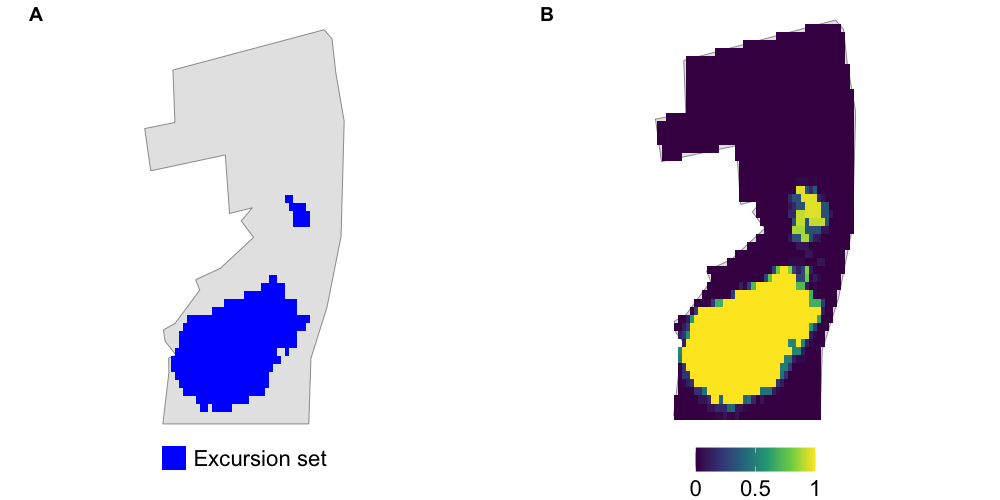
\includegraphics[scale=0.5]{figures/excursions.png}
	\caption{Left:  The positive excursion set with a level corresponding to 1 bird per hectare and probability 0.95.  Right: The positive excursion function with a level corresponding to 1 bird per hectare}
	\label{fig:excursions}
\end{figure}
To visualise multiple such maps we can use the excursion function $F_u^{+}(s) = \sup \{1 - \alpha ; s \in E_{u,\alpha}^+ \}$, which defines for each location largest possible probability $1 -\alpha$ for which that location would be in the excursion set defined using probability $1 - \alpha$.  i.e.  if we allow greater uncertainty, which locations would be included in the excursion set.  The excursion function with a level corresponding to 1 bird per hectare is shown in \autoref{fig:excursions} (right panel).  This figure can also be interpreted naturally.  It shows the largest possible probability for each location to be a member of a set in which the intensity exceeds a threshold simultaneously across all locations in the set. It is clear from the figure that regions on the edge of the excursion set would be included if the $\alpha$ value were allowed to increase slightly.  However, for regions in the north there is essentially no probability level for which those locations would be included in $A_u^{+}(\lambda)$.  
We chose the threshold of 1 bird per hectare and an error probability of 0.05 to demonstrate the approach.  Multiple values for each of these can be considered as a simple extension.


\section{Discussion}

This paper presents a new approach to analysing point transect distance sampling data that incorporates several innovative methods and considers the bulk of an applied statistician's workflow of model specification, inference procedure, model evaluation and communication of results.  Although any of these areas on its own would be substantive enough to be the main focus of a paper, our brief presentation of issues in sequence along with our chosen solutions will be useful to statisticians who face similar questions and data structures.

There are several natural extensions to the model.  For this analysis we only considered a single survey year.  Spatio-temporal extensions to this are possible, for example by considering a space-time interaction models.  \texttt{R-INLA} has the ability to fit space-time effects that can be represented as a Kronecker product of the relevant precision matrices \citep{blangiardo_spatial_2013, yuan_point_2017}.  An example of this type of space-time interaction effect is an interaction between the spatial SPDE with an auto-regressive temporal process.  \cite{blangiardo_spatial_2013} show how this can be done with numerous examples and code snippets.  

Another natural extension is to consider more complicated observation processes.  There is the potential to include explanatory covariates on detection function parameters.  For example, we did not make use of the detection type (audio or visual) in our analysis, although this was recorded and detectability may vary depending on whether a bird is seen or heard.  Other factors could be considered, such as weather conditions, observer expertise, animal behaviour and morphological traits.  Any additional parameters to the non-linear model components will be estimated using the outer-optimisation step of iterated INLA.  [[Can I speculate here about how iterated INLA might perform as parameters are added to non-linear components?  Is, higher-dimensional optimisation slower/infeasible/unstable at a certain point?]]  

The iterated INLA inference procedure is a general approach that could be applied to other non-linear model components that arise in the area of spatial ecology.  We note two promising areas in which our flexible inference procedure may be useful:

\begin{itemize}
	\item \textbf{Selectivity analysis} In surveys of the marine environment, the size, length and weight of fish affects the likelihood of being caught in a trawl net.  Thus any analysis of these data must account for this.  The probability of capture is typically modelled as a logistic function with parameters that depend on morphological traits \citep{herrmann_understanding_2016, madsen_selectivity_2007, galbraith_demersal_1994}, which could be estimated jointly with the spatial distribution within our inference framework.  
	\item \textbf{Functional responses} In the area of understanding species-habitat or species-species interactions, the concept of a `functional response' captures the idea that the abundance of a resource or risk will affect the response to it \citep{holling_some_1959}.  These varying responses can be described mathematically using parametric equations that have the desired properties, e.g. a horizontal asymptote so that beyond a certain threshold no extra amount of a resource will affect the response to it.  These types of responses are typically not considered in species distribution models but our framework allows them to be estimated alongside the more common linear or quadratic fixed effects. This flexibility in specifying model components could also be more widely applicable in areas such as public health and spatial epidemiology, where responses to conditions may be non-linear.  
	
\end{itemize}
We note that many of the themes addressed in this paper apply beyond the field of spatial ecology and will be of interest to the spatial statistics community in general, particularly for applications with complex observation models of latent processes and where spatial predictions are a key output of the analysis

In our analysis we only briefly touch upon the problem of communicating uncertainty in maps and highlight the excursions methods as a new and positive addition to this area.  In our example, the threshold was chosen to illustrate the method but we believe that discussions with relevant stakeholders will lead to agreement on a (possibly large) set of thresholds that are relevant given the aims and context of the analysis.  This requires the input of both the relevant domain experts and statisticians so stakeholders understand the consequences of the thresholds and uncertainty levels they wish to consider.  We also note the potential for excursions to be used to define the notion of occupancy (and thus map occupied areas, with a given probability of error).   

We end with a note on the similarity between what we have done and existing two stage approach.  The one-stage thinned point process perspective can seem fundamentally different to a two-stage GAM approach fitted to count data.  It can be tempting to think that, because the point process model does not require us to bin the data into counts, we can avoid some loss of information.  However, we also made the same assumption of constant intensity within each transect as in more traditional distance sampling approaches.  This leads to the same loss of information since we do not use the exact location of points within each transect, except to account for detectability.

In summary, we have presented a novel framework for analysing point transect distance sampling data that introduces new approaches to model specification, inference procedure and communication of results.  These developments will be of interest to those with similar data structures in spatial ecology as well as researchers in other areas who we hope will explore the full flexibility and generality of these developments in their own work.    

% spp has potential to provide general framework? [Janine comment]
% Mention modelling on sphere is possible without projecting on to R^2?

\clearpage
\bibliographystyle{humannat}
\bibliography{paper}

\end{document}